\chapter{Surveillance Algorithm}


\section{Introduction}
\label{sec:Introduction}

In the realm of robotics, especially for those designed for emergency response and public safety, the implementation of a sophisticated surveillance algorithm is crucial. A fire bot, a type of robot specifically designed for firefighting and scouting in hazardous environments, is a prime example where such an algorithm is not just beneficial, but essential. Surveillance algorithm equips fire bots with the capability to dynamically scan and interpret their surroundings, facilitating real-time decision-making and strategy formulation.

As we talked about in section 2.2, there isn't much detailed research on using these surveillance systems in fire bots. But, there are some methods for exploring unknown places, like Frontier-Based Exploration [3] and RRT Exploration [4], that are similar to what we're trying to do. These methods are a good starting point for us. In this chapter, we're going to look at one of these exploration methods and think about how we can change it to make a surveillance system that fits what fire bots need.

\begin{figure}[h]
  \centering
  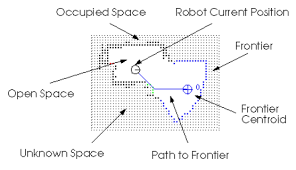
\includegraphics[width=0.9\textwidth, height=0.5\textheight]{Bilder/FBE1.png}
  \caption{Frontier Based Exploration [3]}
  \label{fig:FBE1}
\end{figure}

\begin{itemize}
    \item \textbf{Unknown Region} is the territory that has not been covered yet by the robot’s sensors.
    \item \textbf{Known Region} is the territory that has already been covered by the robot’s sensors.
    \item \textbf{Open-Space} is a known region which does not contain an obstacle.
    \item \textbf{Occupied-Space} is a known region which contains an obstacle.
    \item \textbf{Occupancy Grid} is a grid representation of the environment. Each cell holds a probability that represents if it is occupied.
    \item \textbf{Frontier} is the segment that separates known regions from unknown regions. Formally, a frontier is a set of unknown points that each have at least one open-space neighbor.
\end{itemize}
The terminology described above is shown in Figure.2, shows implementation of Frontier Based Exploration FBE[3] for mapping unknown environments. It utilizes  Wavefront Frontier Detector[7] Algorithm to find frontiers and then use gmapping, that implements Simultaneous Localization and
Mapping (SLAM) [5]and move base [6], a planning algorithm package to plan a path to move to the nearest frontier iteratively till the complete environment is mapped as shown in Figure.3.

\begin{figure}[h]
  \centering
  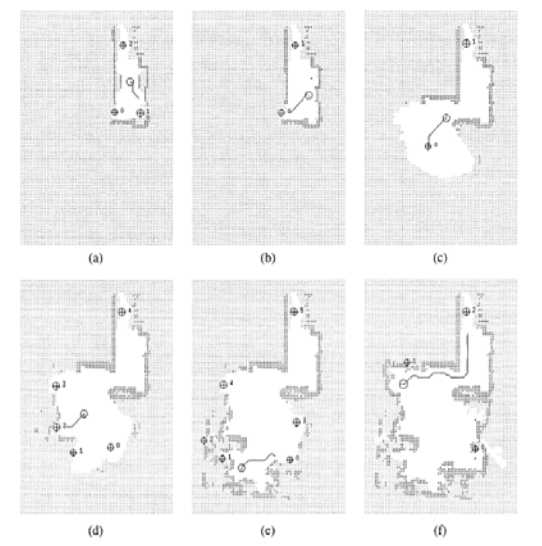
\includegraphics[width=0.9\textwidth, height=0.5\textheight]{Bilder/frontier_grids.png}
  \caption{Occupancy grids during exploration[3]}
  \label{fig:FBE2}
\end{figure}

\section{Approach}
\label{sec:Approach}

In this section, we build upon the insights gained from Section 4.1 about the Frontier-Based Exploration (FBE)  method.We will continue to discuss how we can develop a surveillance algorithm for robots.

In FBE, a key step is choosing the right frontiers. Frontiers are the locations on the occupancy grid that mark the boundary between areas the known region and unknown region. The Wavefront Frontier Detector [7] is used in FBE [3] to pick these frontiers. The robot then chooses the frontier closest to its starting position as its  target goal and uses a path planning algorithm to reach it. By doing this over and over, the robot fully explores the map, updating the occupancy map to show free space and space with obstacles in unknown region.

In our surveillance algorithm for robots, selecting the right frontiers is a key step. Unlike Frontier-Based Exploration (FBE), where any unexplored frontier is a target, our algorithm focuses on choosing frontiers that maximize surveillance coverage. We start with an occupancy map showing free, occupied, and unknown spaces.

\begin{figure}[h]
  \centering
  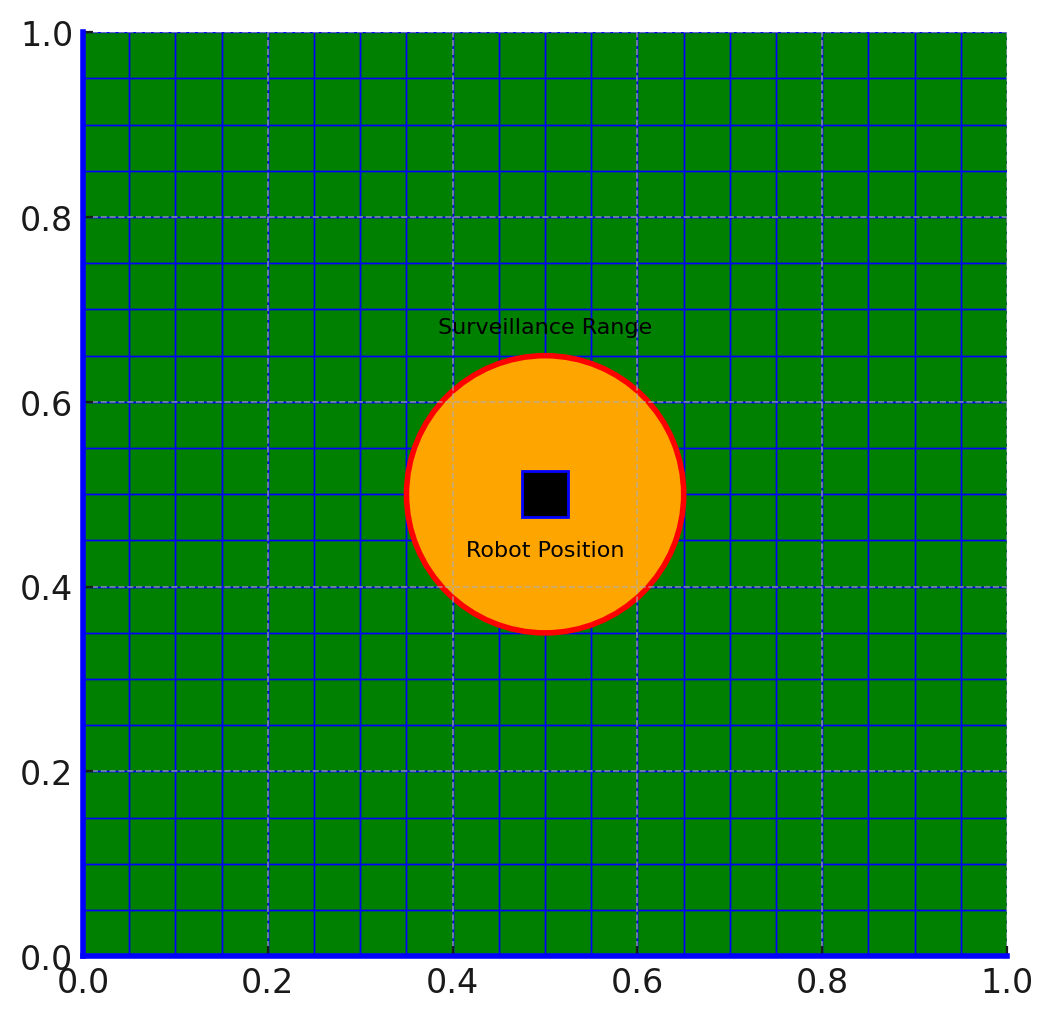
\includegraphics[width=0.7\textwidth, height=0.4\textheight]{Bilder/frontier.png}
  \caption{Frontier Boundary}
  \label{fig:frontier}
\end{figure}

The robot's surveillance range determines the potential frontiers, essentially the areas just beyond what the robot can currently see. We then select a target frontier from these options, prioritizing those that expand the surveillance area the most. This approach ensures that each movement of the robot is strategically made to enhance its surveillance effectiveness, as shown in Figure 4.

This method prioritizes strategic surveillance over mere exploration, choosing target frontiers that offer the greatest increase in monitored area within the robot's visual field.


Description of Figure.4:
\begin{itemize}
    \item \textbf{Explored Region} is the area  that has been covered  by the robot’s sensors (orange region).
    \item \textbf{Surveillance Range} is the range that senor can keep surveillance from robot's position.
    \item \textbf{Free-Space} is a known region which does not contain an obstacle.
    \item \textbf{Occupied-Space} is a known region which contains an obstacle.
    \item \textbf{Occupancy Grid} is a grid representation of the environment. Each cell holds a probability that represents if it is occupied.
    \item \textbf{Frontier} is the segment that separates explored regions from free space Formally.
\end{itemize}


\section{Implementation}
\label{sec:Implementation}

\subsection{Line Of Sight}
\label{sec:line of sight}

In the Frontier-Based Exploration (FBE) algorithm, a significant feature is the Wave Frontier Detection method, which identifies the boundaries between areas already explored and those that are not yet explored. This technique uses laser data to locate new frontiers, guiding the robot to unexplored regions for effective environmental mapping.

Our surveillance algorithm, while drawing inspiration from Wave Frontier Detection, diverges in its core objective to align with the specific demands of surveillance. In contrast to FBE's focus on uncovering unexplored areas, our approach concentrates on maximizing the efficiency of the surveillance area. This is achieved through a Line of Sight approach combined with using the surveillance range as a parameter to assess the area within the vicinity of the robot

\begin{figure}[h]
  \centering
  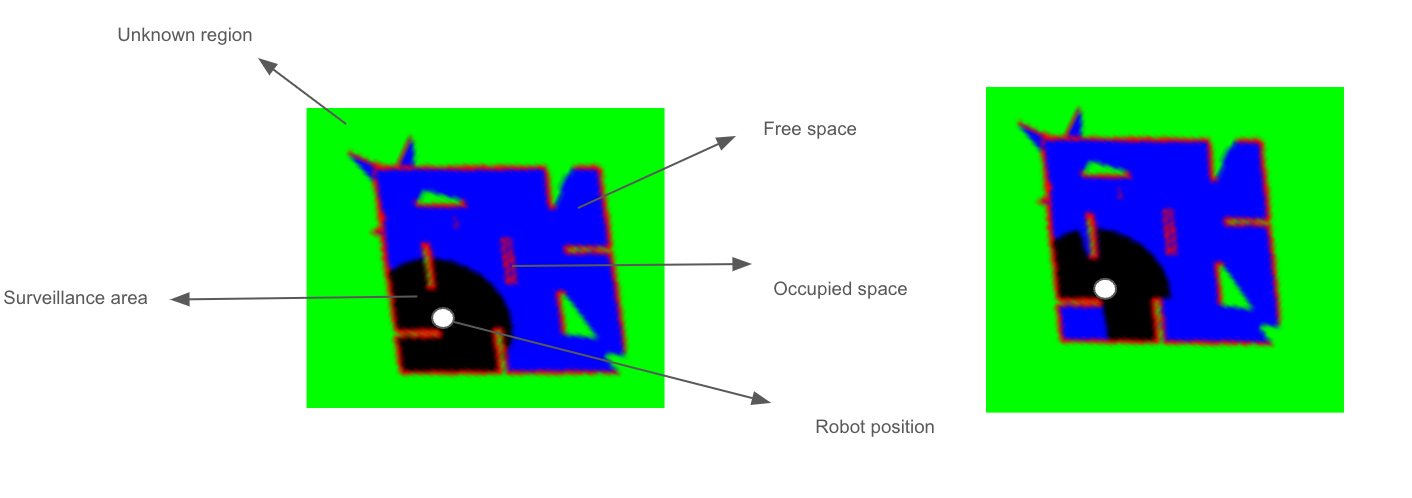
\includegraphics[width=0.7\textwidth, height=0.3\textheight]{Bilder/LOS.png}
  \caption{occupancy grid on left with out line of sight , and on right with line of sight}
  \label{fig:LOS}
\end{figure}

This adapted methodology functions similarly to a laser scan in a WFB. It evaluates the surveillance gain by considering the area within the robot's range, excluding regions obstructed by obstacles. Thus, unlike the FBE where the goal is to identify and move towards unexplored frontiers, our surveillance algorithm prioritizes efficient coverage of the observable area. It ensures that the chosen areas for surveillance are unblocked and within clear sight of the robot’s sensors, enhancing the quality and reliability of the surveillance data collected.





\begin{figure}[H]
\begin{algorithm}[H]
\DontPrintSemicolon
\SetKwFunction{FLineOfSight}{LineOfSight}
\SetKwProg{Fn}{Function}{:}{}
\Fn{\FLineOfSight{grid\_map, start, end, unoccupied\_value}}{
\KwData{Grid map \( grid\_map \), start point \( start \), end point \( end \), value for unoccupied cells \( unoccupied\_value \)}
\KwResult{frontier location if it's in line of sight}
\( x0, y0 \) \(\leftarrow\) start\;
\( x1, y1 \) \(\leftarrow\) end\;
\( dx \) \(\leftarrow\) \( |x1 - x0| \)\;
\( dy \) \(\leftarrow\) \( -|y1 - y0| \)\;
\( sx \) \(\leftarrow\) \textbf{if} \( x0 < x1 \) \textbf{then} \( 1 \) \textbf{else} \( -1 \)\;
\( sy \) \(\leftarrow\) \textbf{if} \( y0 < y1 \) \textbf{then} \( 1 \) \textbf{else} \( -1 \)\;
\( err \) \(\leftarrow\) \( dx + dy \)\;
\While{True}{
    \lIf{\(x0 = x1\) \textbf{and} \(y0 = y1\)}{\Return{True}}
    \lIf{\(grid\_map[x0, y0] \neq unoccupied\_value\)}{\Return{False}}
    \( e2 \) \(\leftarrow\) \( 2 \times err \)\;
    \If{\(e2 \geq dy\)}{
        \( err \) \(\leftarrow\) \( err + dy \)\;
        \( x0 \) \(\leftarrow\) \( x0 + sx \)\;
    }
    \If{\(e2 \leq dx\)}{
        \( err \) \(\leftarrow\) \( err + dx \)\;
        \( y0 \) \(\leftarrow\) \( y0 + sy \)\;
    }
}
\Return{\(x1,y1\)}\;
}
\caption{Function LineOfSight}
\label{alg:line_of_sight}
\end{algorithm}
\end{figure}


\subsection{Gain Function}
\label{sec:gain function}
Gain Function as a key component that evaluates and selects the most advantageous frontier based on the maximization of the surveillance area.

\begin{equation}
F = \{f_1, f_2, \ldots, f_n\} \quad \text{and} \quad G = \{g_1, g_2, \ldots, g_n\}
\end{equation}

Here, \( F = \{f_1, f_2, \ldots, f_n\} \) represents the set of potential frontiers, and \( G = \{g_1, g_2, \ldots, g_n\} \) represents the set of corresponding subgraphs for each frontier.
\begin{equation}
A_i = \left( \sum_{i,j} \left[ g_i[i, j] = \text{s} \right] \right) \times r^2
\end{equation}

Here, \(A_i\) represents the area of each sub graph from each frontier point,  S  represents state of explored  cells in graph, r is the resolution of cell.



\begin{equation}
G(f) = \max_{f \in F} A(f_i)\rightarrow f_i 
\end{equation}


The gain function \(G(f)\) , as articulated through these equations, stands at the core of this surveillance algorithm, intricately balancing the computational efficiency with the operational efficiency of the robot.


\subsection{Putting the Algorithm into Action}
\label{sec:Putting_the_Algorithm_into_Action}

Our surveillance algorithm is a type of Greedy Heuristic, which means it makes the best decision it can at each step, focusing on immediate benefits rather than long-term outcomes. Unlike algorithms that just find the shortest path, our approach aims to find a path that covers the largest surveillance area possible.

Here's how the algorithm works in action:

\textbf{1. Initial Setup and Iterations:}

The algorithm starts with the robot’s initial position as the first frontier. We define a surveillance area using the robot's current position as the center and its surveillance range to determine the boundary. This area is represented in Figure.4. We then use the Line of Sight approach to identify which parts of this area are visible and update our map accordingly, as shown in Figure.5.

\textbf{2. Finding and Evaluating Frontiers:}

In each subsequent iteration, we look for new frontiers just outside the current surveillance area and within the free space. The number of frontiers depends on several factors, including surveillance range, map size, and visibility. For each frontier \( f_i \) in the set \( F = \{f_1, f_2, \ldots, f_n\} \), we create a corresponding sub-graph \( g_i \) in the set \( G = \{g_1, g_2, \ldots, g_n\} \).


\begin{figure}[h]
  \centering
  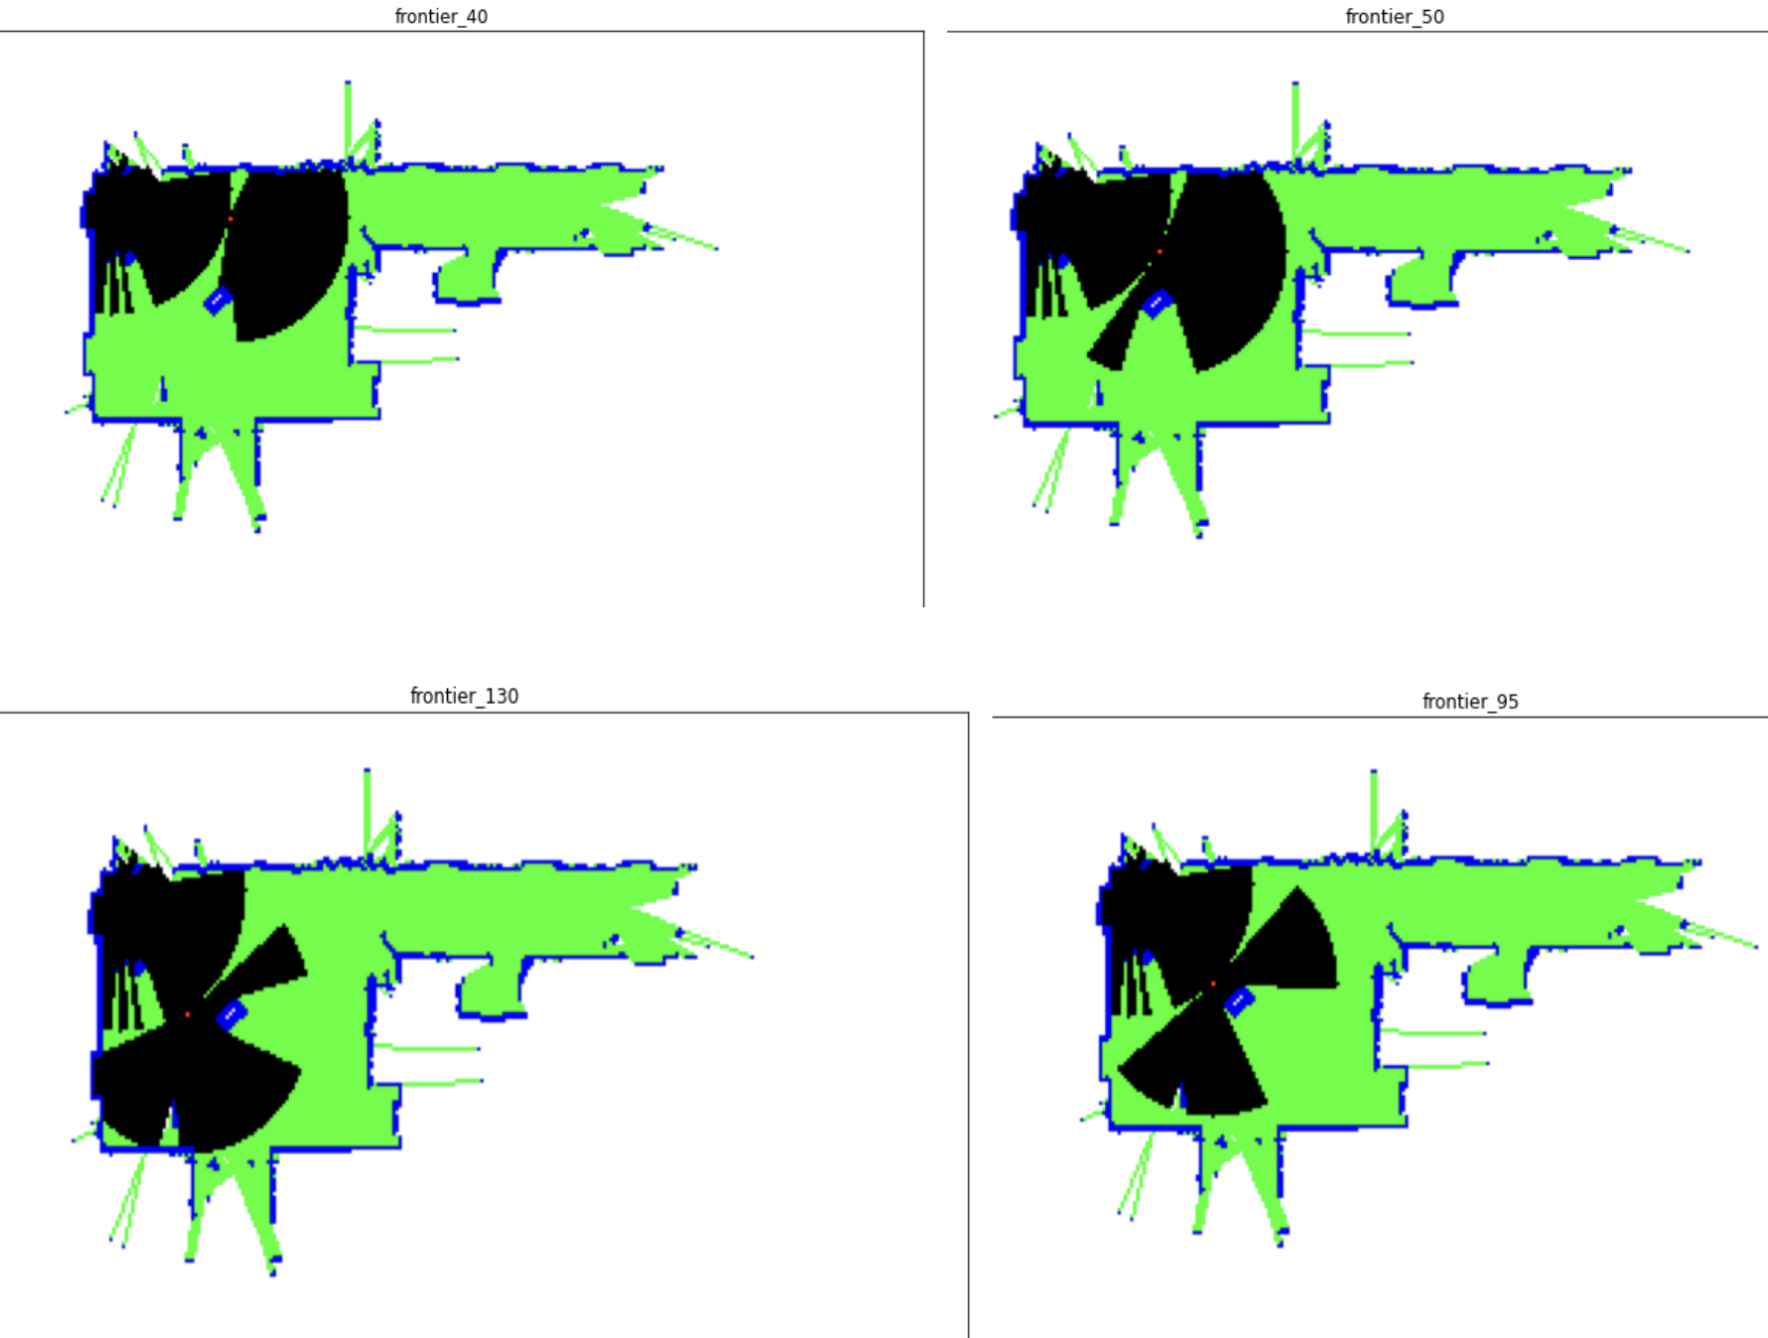
\includegraphics[width=0.9\textwidth, height=0.5\textheight]{Bilder/frontiers.png}
  \caption{Randomly selected sub graphs in iteration - 2 shows  Surveillance area of 4 different frontiers with surveillance range of 4 meters.}
  \label{fig:Frontiers}
\end{figure}


\textbf{3. Applying the Gain Function:}

We apply the gain function to each sub-graph to find the one that offers the largest surveillance area. The selected sub-graph  frontier becomes our next way point, and sub graph is used for the following iteration.

\textbf{4. Repeating the Process:}

This process is repeated until we either reach a predefined number of iterations or cover all the free space, meaning there are no more frontiers left to explore. 

By focusing on maximizing the surveillance area at each step, the algorithm efficiently guides the robot through various way points, ensuring comprehensive coverage of the environment.

\section{Experimental result}

We further tested our algorithm in a real-world setting by creating a map of one of the university's blocks using SLAM (Simultaneous Localization and Mapping). This area, consisting predominantly of free space, spans approximately 110 square meters. We executed our surveillance algorithm on this map to demonstrate its practical effectiveness.


 \begin{figure}[h]
  \centering
  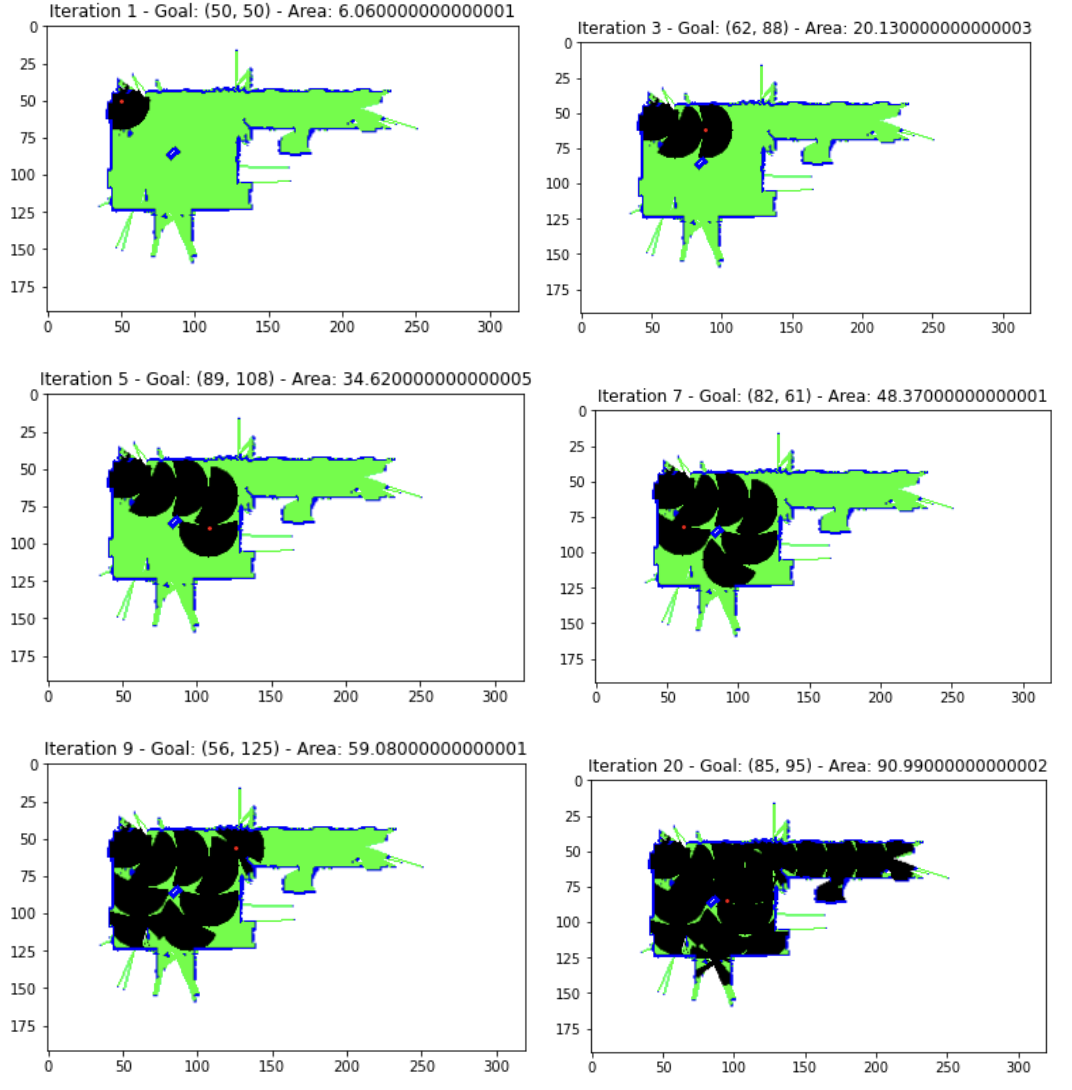
\includegraphics[width=0.7\textwidth, height=0.3\textheight]{Bilder/grid_maps.png}
  \caption{sub graphs at randomly selected iterations}
  \label{fig:LOS}
\end{figure} \

\(Figure 6\) illustrates how our surveillance algorithm covers the area, implementing the concepts discussed in \(Section 4.3\). Additionally, \(Table 1\) provides detailed insights into each iteration of the algorithm, including the area explored, the total number of frontiers identified, and the execution time for both single and multi-process setups. The results indicate that while the Gain Function is computationally intensive, running the algorithm in a multi-process environment is currently recommended for optimal performance.


\label{appendix:Heuristic Goals Estimation}

\begin{table}[ht]
\centering
\begin{tabular}{|c|c|c|c|c|c|}
\hline
Iteration & Goal      & Coverage Area   & Frontiers & CPU (s)  & multi process(s) \\ \hline
1         & (50, 50)  & 6.06            & 1         & 0.2277       
& 1                      \\ \hline
2         & (62, 67)  & 13.08           & 50        & 9.1336                 & 3                      \\ \hline
3         & (62, 88)  & 20.13           & 110       & 19.9720                & 5                      \\ \hline
4         & (68, 108) & 27.37           & 161       & 29.4274                & 8                      \\ \hline
5         & (89, 108) & 34.62           & 228       & 41.5267                & 11                     \\ \hline
6         & (105, 95) & 41.64           & 293       & 53.3847                & 14                     \\ \hline
7         & (82, 61)  & 48.37           & 352       & 64.1778                & 18                     \\ \hline
8         & (103, 61) & 54.09           & 392       & 71.0921                & 20                     \\ \hline
9         & (56, 125) & 59.08           & 414       & 74.8881                & 21                     \\ \hline
10        & (56, 146) & 64.06           & 448       & 80.8565                & 24                     \\ \hline
11        & (56, 167) & 69.61           & 461       & 83.2327                & 26                     \\ \hline
12        & (56, 188) & 74.53           & 488       & 88.0545                & 27                     \\ \hline
13        & (106, 120)& 79.03           & 502       & 90.4957                & 29                     \\ \hline
14        & (56, 209) & 83.05           & 495       & 89.0060                & 28                     \\ \hline
15        & (125, 89) & 86.16           & 501       & 90.0417                & 28                     \\ \hline
16        & (76, 170) & 88.19           & 533       & 95.6528                & 30                     \\ \hline
17        & (49, 104) & 89.01           & 526       & 94.4460                & 29                     \\ \hline
18        & (83, 80)  & 89.76           & 496       & 89.9992                & 28                     \\ \hline
19        & (84, 125) & 90.40           & 456       & 81.7659                & 26                     \\ \hline
20        & (85, 95)  & 90.99           & 431       & 77.2387                & 25                     \\ \hline
\end{tabular}
\caption{Table shows algorithm performance on each iteration for surveillance range of 2 meters on occupancy map in \(Figure.6\)}
\label{table:Table shows coverage area for each iterations, 
 selected frontiers, Exection time on cpu & multi processing}
\end{table} 



\section{Way-Point Optimization}

The approach we have discussed so far for determining way points in a surveillance area is indeed heuristic in nature. This means it aims to make the best possible decision at each step, focusing on immediate benefits rather than considering the entire sequence of actions in a long-term perspective. However, to clarify and refine our objective: our primary goal is to determine an optimal path that maximizes the surveillance area coverage.

In this context, we are not merely looking for a path that connects all designated points or goals. Instead, we are seeking a route that maximizes coverage of the surveillance area while also ensuring the overall path length is minimized. This dual objective requires a careful balancing act between covering as much area as possible and doing so in an efficient manner.

For implementing this optimization, we are employing the Greedy Randomized Adaptive Search Procedure (GRASP)[11]. GRASP is a well-known meta heuristic approach that is particularly effective for solving complex combinatorial problems. It operates in two main phases: a construction phase, where a feasible solution is built using a greedy randomized method, and a local search phase, where this solution is iteratively improved upon.

In the context of our problem, GRASP helps us in systematically exploring different configurations and sequences of way points, thereby enabling us to find a route that strikes the optimal balance between maximizing surveillance area coverage and minimizing travel distance. This approach is especially powerful in scenarios where the search space is large and the optimal solution is not immediately apparent, making it an ideal choice for our Way-Point Optimization task.

Thus, while our method is indeed heuristic, it is strategically designed to yield a solution that is as close as possible to the optimal, given the complexity and constraints of the problem at hand.




\begin{figure}[H]
\begin{algorithm}[H]
\DontPrintSemicolon
\SetKwFunction{FGRASP}{GRASP}
\SetKwFunction{FGreedyRandomizedConstruction}{GreedyRandomizedConstruction}
\SetKwFunction{FLocalSearch}{LocalSearch}
\SetKwFunction{FTwoOptSwap}{TwoOptSwap}
\SetKwFunction{FCalculateTotalDistance}{CalculateTotalDistance}
\SetKwProg{Fn}{Function}{:}{}
\Fn{\FGRASP{Goals, Alpha, MaxIterations}}{
\KwData{List of goals \( Goals \), randomness factor \( Alpha \), maximum number of iterations \( MaxIterations \)}
\KwResult{The best route found to cover all goals}

\For{k $\gets$ 1 \KwTo MaxIterations}{
    Solution $\gets$ \FGreedyRandomizedConstruction{Goals, Alpha}\;
    Solution $\gets$ \FLocalSearch{Solution}\;
    Cost $\gets$ \FCalculateTotalDistance{Solution}\;
    \If{Cost < BestCost}{
        BestSolution $\gets$ Solution\;
        BestCost $\gets$ Cost\;
    }
}
\Return{BestSolution}\;
}
\caption{Greedy Randomized Adaptive Search Procedure (GRASP)}
\end{algorithm}
\end{figure}

The GRASP (Greedy Randomized Adaptive Search Procedure) function orchestrates the overall process of finding an optimal path. It iteratively constructs a random solution using a greedy approach, then refines it through local search. The best solution across all iterations is returned as the final best path in \(Heuristic 3\)

\(Heuristic 4\) This is Greedy Randomized Construction function creates an initial solution by sequentially adding goals to the path. It evaluates and ranks possible next steps by their proximity, but introduces randomness by selecting from the top candidates, not just the nearest, which prevents the algorithm from being trapped in local optima.


\begin{figure}[H]
\begin{algorithm}[H]
\DontPrintSemicolon
\SetKwFunction{FGreedyRandomizedConstruction}{GreedyRandomizedConstruction}
\SetKwProg{Fn}{Function}{:}{}
\Fn{\FGreedyRandomizedConstruction{Goals, Alpha}}{
\KwData{List of goals \( Goals \), randomness factor \( Alpha \)}
\KwResult{A randomly constructed route}

CurrentPosition $\gets$ Goals[0]\;
Solution $\gets$ \{CurrentPosition\}\;
RemainingGoals $\gets$ Goals[1..end]\;
\While{RemainingGoals is not empty}{
    Distances $\gets$ list of distances from CurrentPosition to each point in RemainingGoals\;
    Sort Distances\;
    TopCandidates $\gets$ first Alpha percent of Distances\;
    Chosen $\gets$ randomly select a pair from TopCandidates\;
    Solution $\gets$ Solution + \{Chosen.Goal\}\;
    Remove Chosen.Goal from RemainingGoals\;
    CurrentPosition $\gets$ Chosen.Goal\;
}
\Return{Solution}\;
}
\caption{Greedy Randomized Construction Function}
\end{algorithm}
\end{figure}

The Local Search function takes an initial route and iteratively improves it. It uses the 2-opt swap strategy, which tries exchanging two legs of the route to see if a shorter overall distance can be achieved. This process repeats until no further improvements can be made  \(Heuristic 5\)




\begin{figure}[H]
\begin{algorithm}[H]
\DontPrintSemicolon
\SetKwFunction{FLocalSearch}{LocalSearch}
\SetKwFunction{FTwoOptSwap}{TwoOptSwap}
\SetKwFunction{FCalculateTotalDistance}{CalculateTotalDistance}
\SetKwProg{Fn}{Function}{:}{}
\Fn{\FLocalSearch{Solution}}{
\KwData{Initial route \( Solution \)}
\KwResult{An improved route after applying local search}

BestRoute $\gets$ Solution\;
BestCost $\gets$ \FCalculateTotalDistance{BestRoute}\;
Improved $\gets$ true\;
\While{Improved}{
    Improved $\gets$ false\;
    \For{i $\gets$ 1 \KwTo length(BestRoute)-2}{
        \For{k $\gets$ i+1 \KwTo length(BestRoute)}{
            NewRoute $\gets$ \FTwoOptSwap{BestRoute, i, k}\;
            NewCost $\gets$ \FCalculateTotalDistance{NewRoute}\;
            \If{NewCost < BestCost}{
                BestRoute $\gets$ NewRoute\;
                BestCost $\gets$ NewCost\;
                Improved $\gets$ true\;
            }
        }
    }
}
\Return{BestRoute}\;
}
\caption{Local Search Function}
\end{algorithm}
\end{figure}



\begin{figure}[h]
  \centering
  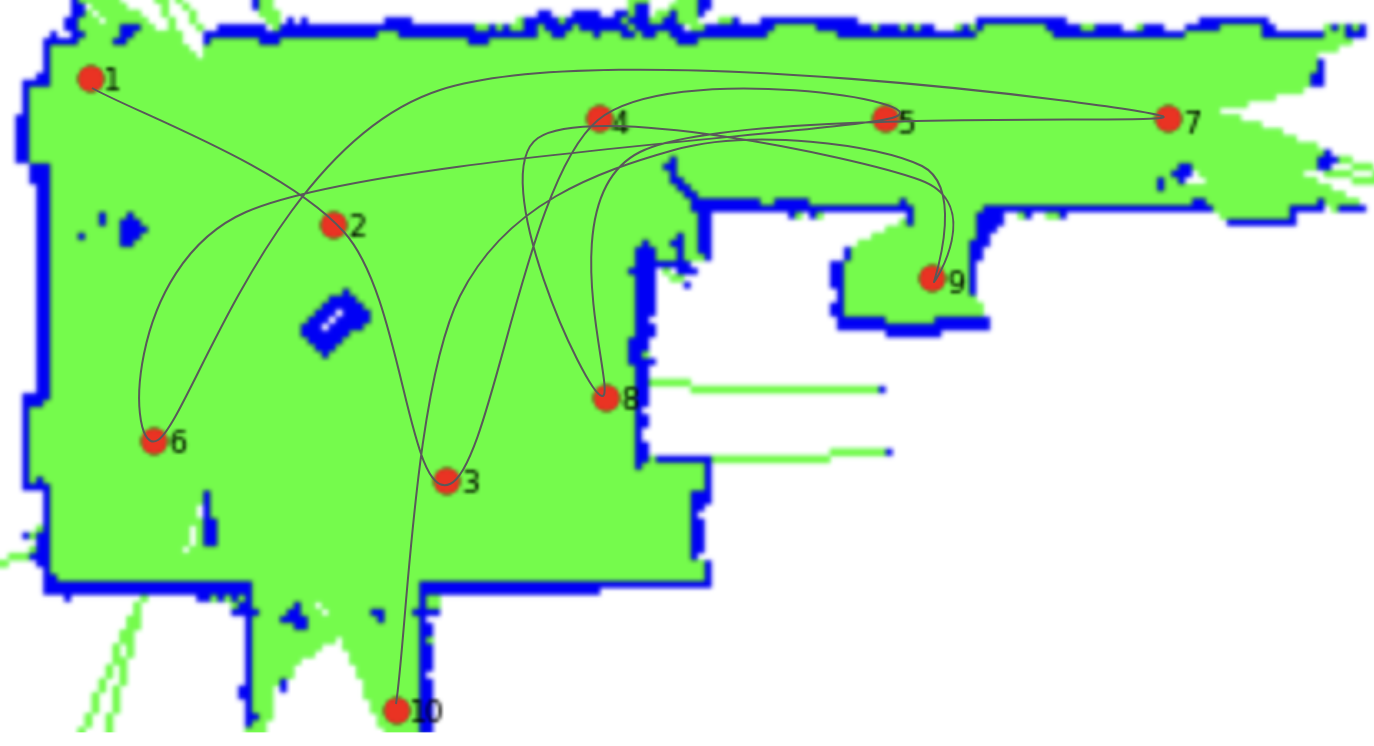
\includegraphics[width=0.7\textwidth, height=0.3\textheight]{Bilder/without_wpo.png}
  \caption{Path without way-point optimization (WPO) which maximizes surveillance area}
  \label{fig:waypoints without waypoint optimization (WPO) only maximizes surveillance area}
\end{figure}


\begin{figure}[h]
  \centering
  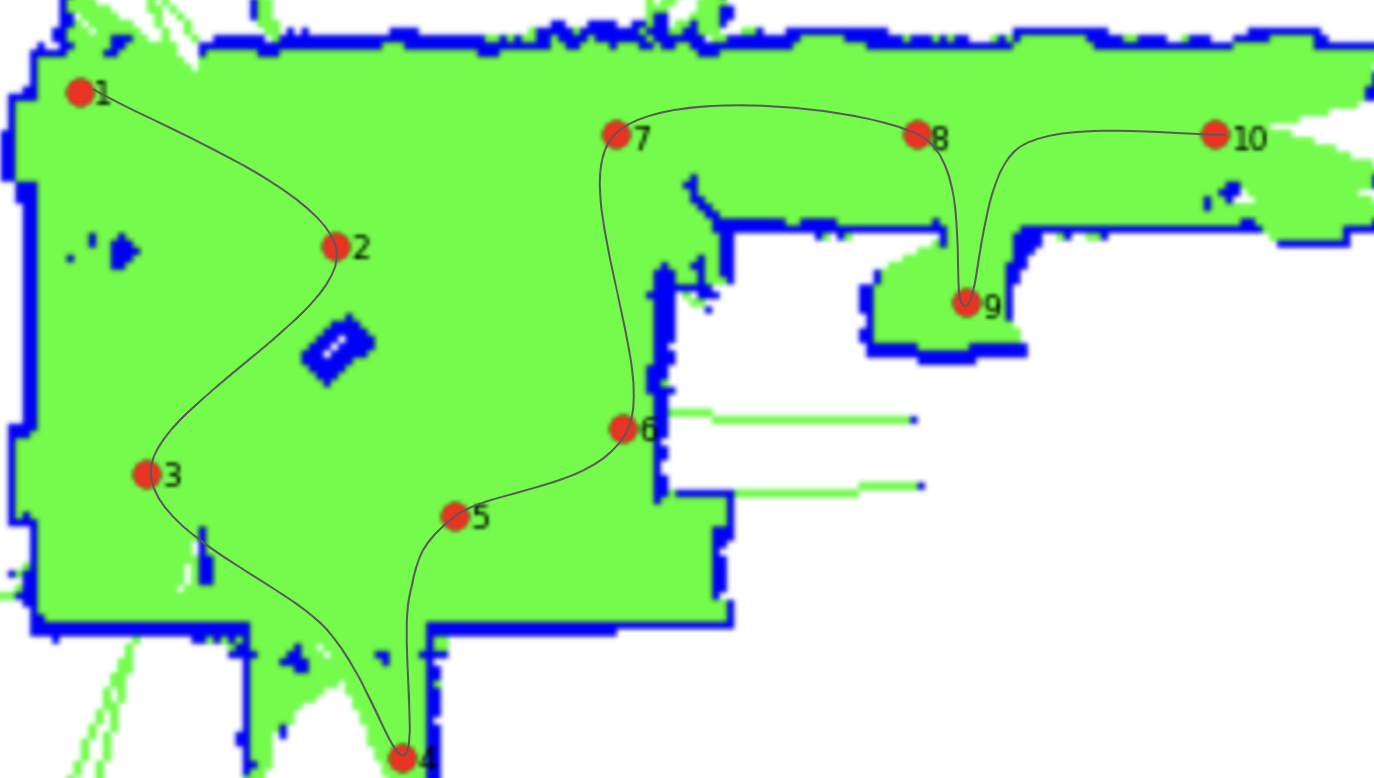
\includegraphics[width=0.7\textwidth, height=0.3\textheight]{Bilder/with_wpo.png}
  \caption{Path with way-point optimization (WPO) which maximizes surveillance area}
  \label{fig:waypoints with waypoint optimization (WPO) which also optimizes path that maximizes surveillance area}
\end{figure}











